\documentclass[11pt,a4paper,twoside]{article}
\usepackage{tascar}
\pagenumbering{arabic}
\pagestyle{empty}
\showtutorialtrue
\begin{document}
\setcounter{tutorial}{1}
\begin{tutorial}{Interfacing from MATLAB/GNU Octave for adaptive measurements}{Darklab + Seminar room}
  In this tutorial you will learn how to control \tascar{} from MATLAB or GNU Octave. 
  %
  You will learn how to (automatically) change \tascar{} parameters from MATLAB/GNU Octave and how to start, stop or rewind the playing back of a scene. 
  %
  At the end you will have a setup of an adaptive measurement procedure, e.g., minimum audible angle in spatially complex masking environments.

  \begin{learnitems}
  \item Change simulation parameters from MATLAB/GNU Octave
  \item Control the playback/time line of a scene
  \end{learnitems}

  \begin{appitems}
  \item Psycho-acoustic measurements in virtual acoustics
  \end{appitems}

  \centerline{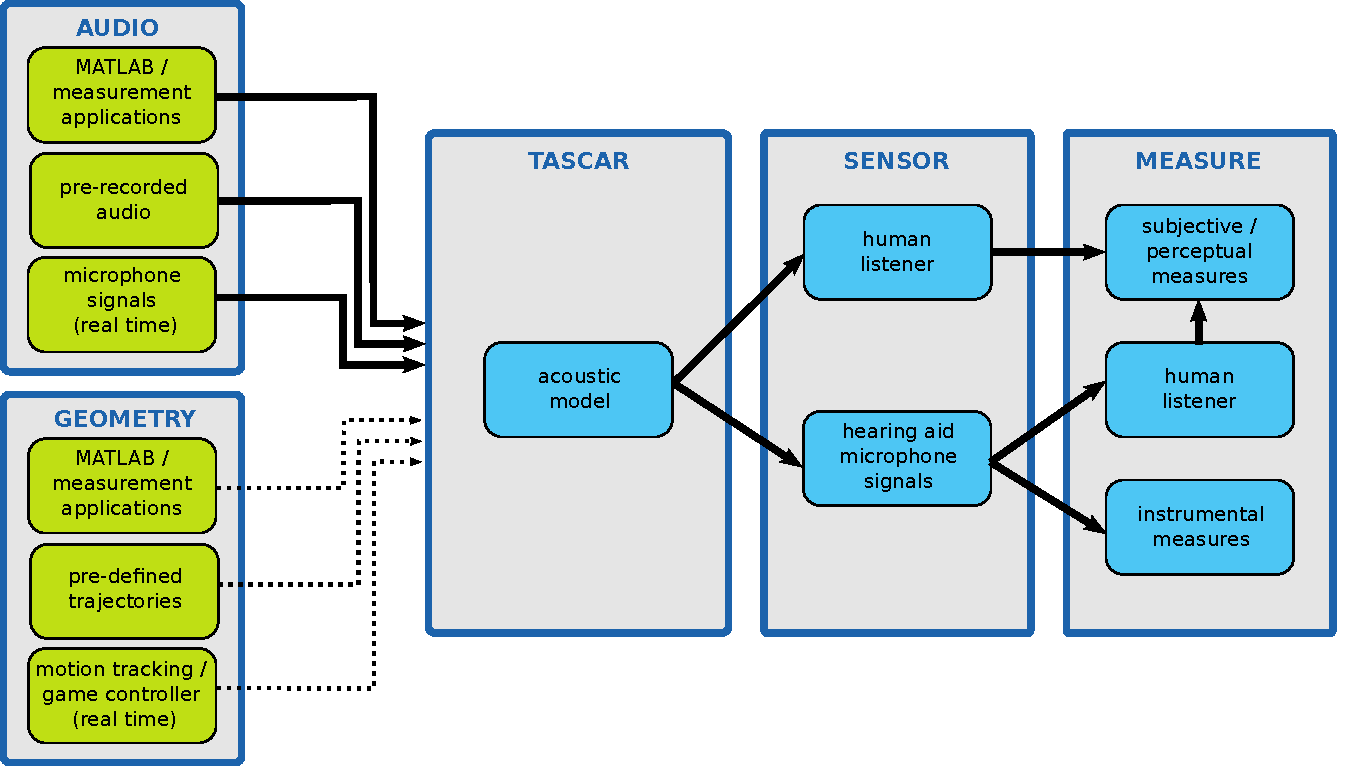
\includegraphics[width=0.8\columnwidth]{applications}}
\end{tutorial}

\ifshowtutorial

\newpage

\subsection*{Part I: loading, closing, generating a scene, modifying OSC variables}
\begin{itemize}

\item Open script \verb!task2_example1_1.m! in MATLAB (or GNU Octave) and your own copy of a file \verb!task2_basic1.tsc! in text editor. (To open MATLAB type  \verb!matlab &! in a terminal) 

\item Using \verb!task2_example1_1.m! load \verb!task2_basic1.tsc! in \tascar{}. 

\item In the \tascar{} window go to \verb!View !$\rightarrow$\verb! OSC variables!. What are the OSC variables you can access? 

\item Using \verb!task2_example1_1.m! play with changing the scene variables and with playing/recording the scene from MATLAB.

\item Open script \verb!task2_example1_2.m! in MATLAB. 

\item Using \verb!task2_example1_2.m! generate a new \tascar{}
  scene. Open this scene in text editor and load in \tascar{} to see
  what you have generated.

\item Try to modify the osc parameters of the new generated scene from
  MATLAB, try playing back and recording for this scene.
\end{itemize}
\subsection*{Part II: modifying xml document, offline rendering}
\begin{itemize}

\item Load \verb!task2_basic2.tsc! to tascar and have a look at the corresponding scene definition file. 

\item Using \verb!task2_example2.m! modify scene \verb!task2_basic2.tsc! (Here you learn to modify the xml document offline). Open both unomdified and modified scene definition in text editor and in \tascar{} to see and hear what you have changed.

\item Using \verb!task2_example2.m! render the static impulse response and image source model of the modified and unmodified scene - you can compare your rendered signals. heeelp

\end{itemize}
\subsection*{Part III: AFC experiment}
\begin{itemize}

\item Design your own AFC experiment with \tascar{} and \tascar{}
  MATLAB tools. Can you measure MAA in noise as a function of noise
  direction? Or spatial release from masking?

  You may use our AFC toolbox. Type \verb!afcgui maa subjectid! in
  MATLAB to start an example measurement (MAA).  Modify functions
  \verb!afccfg_maa.m! and \verb!afc_maa_play_interval.m! to fit your
  needs.

\end{itemize}

\fi
\end{document}
